\documentclass[12pt,a4paper]{book}
%\usepackage[utf8]{inputenc}
\usepackage{tongji}


\begin{document}
	
	\title{\erhao\hei 
	软管组件纤维编织增强层非线性本构关系研究及实验测试
	}
\author{
	胡牧原
	}
\maketitle

	\tableofcontents
	
\begin{abstract}
基于Hachemi提出的金属编织层本构理论以及拉伸实验的研究方法,进行了不同尺寸金属编织软管的拉伸实验。发现金属编织层在拉伸时会出现强烈的结构非线性,而该理论不能在非线性段与实验结果相吻合。提出了对理论中编织层刚度矩阵修正方法,将金属纤维间交叠产生的接触等效地转化为“修正基体”(Modified Matrix Method),独立于金属纤维自身产生的刚度。同时,结合编织角在实验中呈现的变化趋势,提出了以下假设:管状金属编织层在等位移拉伸荷载下编织角呈线性变化。这是与Hachemi的假设恰好相反的:Hachemi认为编织层受拉时,编织角减小到一定程度时会发生锁定现象,而实验证明了编织角并不会发生锁定,且直到编织层破坏为止,编织角变化的趋势基本呈线性。还提出了修正编织角变化的加速系数k,通过金属纤维间的侧向接触解释了实验与数值仿真结果中,力位移曲线与编织角变化曲线不能同时吻合的力学机理。

we conducted an experiment and put forward several modifications, based on the method proposed in Hachemi’s research of metal wire braid reinforced hose, in order to enhance the constitutive theory, which is discovered not keeping up with the experimental results when it shows far more non-lineal mechanical behavior than the theory predict. We introduced a “modifying matrix”, from composites mechanics, to detach inter-wire contacts from wire elongation, seldom considered before. We also proposed a hypothesis opposite to Hachemi’s: the hose’s braid angle decreased linearly, applied displacement load with constant loading rate, rather than locked at a certain degree. So that we introduce a modification coefficient k, accelerating the decrease of braid angle to match the linearity in force-displacement curve. Lateral contact is considered to be the factor of excessively decreased braid angle when the calculated curve perfectly meet the experimental one, with suitable k.

Key Words:Braid,Hose,modification, 
\end{abstract}



	\chapter{引~言}

\section{}

金属编织加强软管在工程中有着非常广泛的应用,其结构如图\ref{intro}所示,是液压传动系统中非常重要的组成部分。因其可以承受相对较大的内压、轴向荷载,同时保持较小的质量、弯曲刚度[1],带来以下优势:可以减小系统的刚度,吸收液压源产生的振动;安装方式灵活,节约了系统内部的空间。
目前对金属编织加强软管的研究,多见于汽车工业中的中刹车管[2]、转向传动管[3]、空调管[4] 等。






\begin{figure}[t]
\begin{tabularx}{5in}{ccc}
\begin{minipage}[t]{2in}
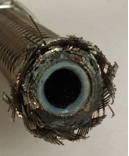
\includegraphics[width=1.5in]{hose-1}
\end{minipage}
\begin{minipage}[t]{2in}
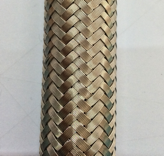
\includegraphics[width=1.5in]{hose-2}
\end{minipage}
\end{tabularx}
\begin{minipage}[t]{2in}

\includegraphics[width=1.5in]{unit-1}
\end{minipage}

\caption{This is a caption}
\label{intro}

\end{figure}







对软管加强层理论的研究,基本使用通过加强层的总体的要是通过软管理论主要有两个分支[5]:一种是加强层含量较低,橡胶管起主要作用的软管,由Kuipers等人[6,7]提出并完善,适用于帘线加强的软管;另一种是编织加强层主要承力的软管,主要研究的是钢丝螺旋缠绕加强层。软管轴向受拉时,缠绕的金属丝会沿缠绕方向“流动”。编织加强层仅作为螺旋缠绕的一种特例:两层缠绕方向相反,且不允许“流动”的缠绕层[5]。
近20年对编织加强结构的研究主要集中在复合材料编织。复合材料纤维编织的与金属纤维编织的传力机制差别非常明[8]:复合材料纤维只承受单向应力;而金属编织层中的金属丝间的接触关系会直接影响编织层整体的传力,不能忽视。因此,并没有至今尚没有成熟、独立,考虑金属丝间接触关系的编织加强层理论。
有学者尝试用连续介质力学的基本理论推导编织层的本构,如Evans[5]编织层金属纤维侧向传力机制,Horgan等人[9] 提出了纤维加强材料的应变能密度函数,国内学者计算了编织结构强度与突加荷载的情况[10,11]。但主流的研究办法还是结合实验,提出能够反映加强层力学行为的有限元模型。Wijaya[4]对包含软管各层材料及编织层的试件进行了压缩实验,认为金属编织层的应力应变关系是线性的,在软管整体动态特性的研究中取得了较好的效果。Cho[3]研究了编织层在扣压安装接头中的力学行为,结合压缩实验提出了弹塑性的本构模型,Rattensperger[8]同样针对压缩的过程,编织层厚度方向引入一组等效非线性弹簧,表征金属纤维间相互作用。
Hachemi[12]对编织层进行了拉伸试验,将复合材料编织中考虑材料非线性行为的特征单元法(首先由Reese[13]提出)引入金属编织层的研究,提出了能够反映编织结构编织角变化的本构模型。该模型将编织层简化两层Rebar单元,只在编织方向上有刚度。但该模型仍然没有考虑两层Rebar单元之间相互接触的关系。
本研究实验表明,Hachemi[12]本构模型的非线性行为并不足够强,不能与本研究中的高压金属编织加强软管的拉伸实验结果相吻合。我们试图通过引入金属纤维间的接触关系来修正该理论与实验的差距。使得包括非线性段的实验结果都能够与修正后的理论值相吻合。



	
	

	\chapter{软管拉伸试验}



	
	\chapter{修正刚度}
	\chapter{强度理论}


	
	
	
	软管组件纤维编织增强层非线性
本构关系研究及实验测试
 




 


绪论
研究背景
金属编织加强软管在工程中有着非常广泛的应用,其结构如图1所示,是液压传动系统中非常重要的组成部分。因其可以承受相对较大的内压、轴向荷载,同时保持较小的质量、弯曲刚度[1],带来以下优势:可以减小系统的刚度,吸收液压源产生的振动;安装方式灵活,节约了系统内部的空间。
软管组件结构
金属编织加强软管由金属编织层分为内管,以及软管组成(如图 1(a)),部分耐高压型号还有额外的螺旋缠绕加强层。软管工作时,绝大部分内压荷载由金属编织层承担,PTFE内管主要起通道的作用,体现其耐腐蚀抗老化的特性。编织加强层由编织机缠绕于内管之上:若干根金属纤维穿过编织机锭子合为一股,由锭子携带,在圆周上的相互穿插交叠形成编织层。
金属编织软管一般采用2×2的编织(twill)形式(如图 1(c)),这是因为金属纤维一般刚度较大,这种编织形式中每股纤维的曲率较小,可以减小金属纤维所受的应力。

 	 	 
					
图 1 编织层加强软管结构。a)软管横截面,b)编织层整体结构,c)2×2编织结构特征单元
Figure 1Structure of Braid Reinforced Hose. a) Section of hose assembly, b)Overall structure of braid layer, c) Representative cell of Twill (2×2 braid)
研究现状
目前对金属编织加强软管的研究,多见于汽车工业中的中刹车管[2]、转向传动管[3]、空调管[4]等。对软管加强层理论的研究,基本使用通过加强层的总体的要是通过软管理论主要有两个分支[5]:一种是加强层含量较低,橡胶管起主要作用的软管,由Kuipers等人[6,7]提出并完善,适用于帘线加强的软管;另一种是编织加强层主要承力的软管,主要研究的是钢丝螺旋缠绕加强层。软管轴向受拉时,缠绕的金属丝会沿缠绕方向“流动”。编织加强层仅作为螺旋缠绕的一种特例:两层缠绕方向相反,且不允许“流动”的缠绕层[5]。
近20年对编织加强结构的研究主要集中在复合材料编织。复合材料纤维编织的与金属纤维编织的传力机制差别非常明[8]:复合材料纤维只承受单向应力;而金属编织层中的金属丝间的接触关系会直接影响编织层整体的传力,不能忽视。因此,并没有至今尚没有成熟、独立,考虑金属丝间接触关系的编织加强层理论。
有学者尝试用连续介质力学的基本理论推导编织层的本构,如Evans[5]编织层金属纤维侧向传力机制,Horgan等人[9]提出了纤维加强材料的应变能密度函数,国内学者计算了编织结构强度与突加荷载的情况[10,11]。但主流的研究办法还是结合实验,提出能够反映加强层力学行为的有限元模型。Wijaya[4]对包含软管各层材料及编织层的试件进行了压缩实验,认为金属编织层的应力应变关系是线性的,在软管整体动态特性的研究中取得了较好的效果。Cho[3]研究了编织层在扣压安装接头中的力学行为,结合压缩实验提出了弹塑性的本构模型,Rattensperger[8]同样针对压缩的过程,编织层厚度方向引入一组等效非线性弹簧,表征金属纤维间相互作用。
Hachemi[12]对编织层进行了拉伸试验,将复合材料编织中考虑材料非线性行为的特征单元法(首先由Reese[13]提出)引入金属编织层的研究,提出了能够反映编织结构编织角变化的本构模型。该模型将编织层简化两层Rebar单元,只在编织方向上有刚度。但该模型仍然没有考虑两层Rebar单元之间相互接触的关系。
研究内容
本研究实验表明,Hachemi[12]本构模型的非线性行为并不足够强,不能与本研究中的高压金属编织加强软管的拉伸实验结果相吻合。我们试图通过引入金属纤维间的接触关系来修正该理论与实验的差距。使得包括非线性段的实验结果都能够与修正后的理论值相吻合。
 
PTFE金属编织加强软管拉伸试验及分析
概述
Hachemi[12]在其对编织加强波纹管的研究中,为了建立金属编织层的有限元模型,利用拉伸试验对其本构理论进行了初步的探索。本研究借鉴了其思路,对几组结构不同的高密度金属编织塑料软管试件进行拉伸试验。试验试件为某型PTFE金属编织加强软管组件,由上海市塑料研究所提供。
软管组建重要参数
根据文献确定实验中需要测量的重要参数。
编织角
编织角(braid angle)是金属编织加强层中极为重要的一个参数。薄壁圆筒理论可以推导出编织结构的平衡[15]角为arctan√2=54.2°,即编织层保持平衡角时,在内压荷载作用下,环向应力等于轴向应力。
 	 	 
图 2编织角及覆盖系数
Figure 2 braid angle and cover factor
覆盖系数

%由于金属纤维相互穿插,编织层中各股纤维一般不能紧密贴合,其间会留下一定空隙,空隙越大,则编织层中金属纤维体积分数越少。文献中将除去孔隙面积的部分占编织层总表面积的比率定义为覆盖系数(cover factor)[14]。取特征单元(如图 2),覆盖系数ξ=1-S_ABC/S_DEF ,
%	 	(1)
%其中,N_s为总股数,N_w为每股金属纤维数,ϕ单根金属纤维直径,D编织层外径,α为编织角。编织层环向特征单元个数为N_S⁄2,则特征单元宽度AC为2πD⁄N_S 。

文献理论及结果
第一组试验
试验试件及设备
试验结果
第二组试验
试验试件及设备
试验结果

第三组试验
试验试件及设备
试验结果

对比与分析
本章小结
金属编织增强层等效刚度修正方法研究
概述
理论模型
本章小结
金属编织增强强度理论研究
概述
3组试验
本章小结
编制增强软管组件爆破压力条件下准静态强度分析

结论与展望
结论
展望

	
	
\end{document}